\section{Architecture}\label{sec:architecture}

The architecture of \SYS{} comprises a combination of two different types of base components: \textsf{worker} and \textsf{router}.
A \textsf{worker} component continuously listens for incoming data by means of non-blocking I/O.
As soon as data flows in, an application-dependent business logic is applied.
A typical use-case is the deployment of a classic filter/map/reduce pattern from the functional programming paradigm~\cite{bird_introduction_1988}.
In such a case, worker nodes execute only one function, namely \texttt{map}, \texttt{filter}, or \texttt{reduce}.
A \textsf{router} component acts as a message broker between workers in the pipeline and transfers data between them according to a given \emph{dispatching policy}.
Figure~\ref{fig:architecture_pipeline} depicts a possible implementation of this dataflow pattern using the \SYS{} middleware.

\begin{figure*}[!t]
  \centering
  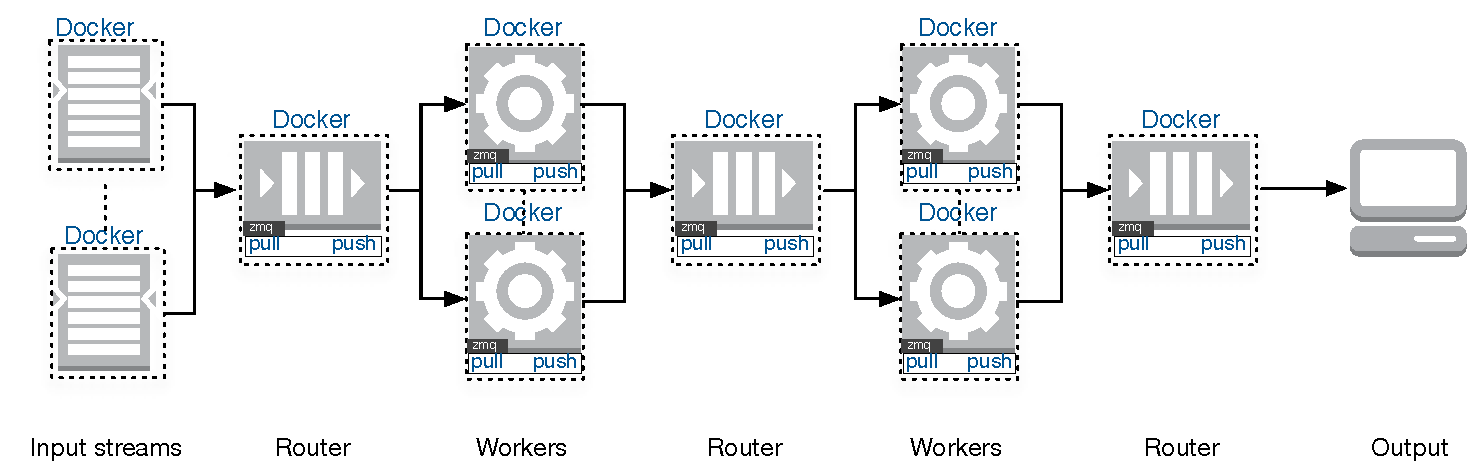
\includegraphics[width=\linewidth]{images/architecture_pipeline}
  \caption{Example of \SYS{} pipeline architecture.}
  \label{fig:architecture_pipeline}
\end{figure*}


\SYS{} is designed to support the processing of sensible data inside SGX enclaves.
As explained in the previous section, the \emph{enclave page cache} (EPC) is currently limited to $128\,MB$.\footnote{Future releases of SGX might relax this limitation~\cite{mckeen2016intel}.}
To overcome this limitation, we settled on a lightweight yet efficient embeddable runtime, based on the \textsc{Lua} virtual machine (\textsc{LuaVM})~\cite{ierusalimschy_luaextensible_1996} and the corresponding multi-paradigm scripting language~\cite{lualang}.
The \textsc{Lua} runtime requires only few kilobytes of memory, it is designed to be embeddable, and as such it represents an ideal candidate to execute in the limited space allowed by the EPC.
Moreover, the application-specific functions can be quickly prototyped in \textsc{Lua}, and even complex algorithms can be implemented with an almost 1:1 mapping from pseudo-code~\cite{leonini2009splay}.
We provide further implementation details of the embedding of the \textsc{LuaVM} inside an SGX enclave in Section~\ref{sec:implementation}.

%\rp{I would argue that the choice of Lua is not actually to overcome the memory limitation. I guess the majority of script interpreters would fit easily inside the 90MB. Besides, *ideal* is a quite strong claim. Of course we do need a script language since we cannot link code dinamically, but I would rather go with the programability arguments, the availability of RxLua, besides of course being easily embeddable and tiny.}

%If a process exceeds the available memory, an encrypted pagination mechanism leads to performance leaks.
%Thus \textsc{SecureStreams} has been designed to use a Lua runtime.
%Lua is a lightweight multi-paradigm programming language designed primarily for embedded systems and clients\cite{ierusalimschy_luaextensible_1996}.
%Its runtime requires only few KB of memory, and thus fits easily in EPC.

Each component is wrapped inside a lightweight Linux container (in our case, the \emph{de~facto} industrial standard Docker~\cite{docker}).
Each container embeds all the required dependencies, while guaranteeing the correctness of their configuration, within an isolated and reproducible execution environment.
By doing so, a \SYS{} processing pipeline can be easily deployed without changing the source code on different public or private infrastructures.
For instance, this will allow developers to deploy \SYS{} on Amazon EC2 container service~\cite{awsec2container}, where SkyLake-enabled instances will soon be made available~\cite{amazonskylake}, or similarly to Google compute engine~\cite{gceskylake}.
The deployment of the containers can be transparently executed on a single machine or a cluster, using a Docker network and the Docker Swarm scheduler~\cite{docker:swarm_2016}.
%\rp{Does Amazon offer machines with Skylake processors with EPC enabled?}
%\ah{It's planned: https://aws.amazon.com/fr/about-aws/whats-new/2016/11/coming-soon-amazon-ec2-c5-instances-the-next-generation-of-compute-optimized-instances/ but we don't know if SGX will be enabled. Google intends also: http://fortune.com/2017/02/24/google-intel-cloud-chip/. Do we have to cite there references?}

The communication between workers and routers leverages \zmq{}, a high-performance asynchronous messaging library~\cite{zero_mq}.
Each router component hosts inbound and outbound queues.
In particular, the routers use the \zmq's pipeline pattern~\cite{zero_mq:pipeline} with the \textsc{Push}-\textsc{Pull} socket types. 
%\rp{Is 'protocol' the best definition? I would rather call it a 'pattern'}\ah{It is, this is one of the different protocols of communication implemented in ZMQ, like explained in the target of the given pointer}\rp{The pointer does not mention protocol to refer to that. push/pull refers to the role of socket endpoints. It is not an agreement on format and content of exchanged messages, as a 'protocol' would be best understood by a common reader.}

The inbound queue is a \textsc{Pull} socket.
The messages are streamed from a set of anonymous\footnote{\emph{Anonymous} refers to a peer without any identity: the server socket ignore which worker sent the message.} \textsc{Push} peers (\emph{e.g.}, the upstream workers in the pipeline).
The inbound queue uses a fair-queuing scheduling to deliver the message to the upper layer.
Conversely, the outbound queue is a \textsc{Push} socket, sending messages using a round-robin algorithm to a set of anonymous \textsc{Pull} peers---\emph{e.g.}, the downstream workers.

% \vs{if there is time, it could be useful to have a drawing that zooms into this aspect of the architecture, not the full pipeline}
This design allows us to dynamically scale up and down each stage of the pipeline in order to adapt it to application's needs or the workload.
Finally, \zmq{} guarantees that the messages are delivered across each stage via reliable TCP channels.
%The pattern is mostly reliable insofar as it will not discard messages unless a node disconnects unexpectedly.
%This fire-and-forget messaging is a messsaging pattern in which we do not expect a direct response to the message, as opposed to request-response protocols\cite{voelter_patterns_2003}.
% The absence of response to a message provides some relevant performances.

We define the processing pipeline components and their chaining by means of Docker's Compose~\cite{docker:compose} description language.
Listing~\ref{pipeline-desc} reports on a snippet of the description used to deploy the architecture in Figure~\ref{fig:architecture_pipeline}.
Once the processing pipeline is defined, the containers must be deployed on the computing infrastructure.
We exploit the \texttt{constraint} placement mechanisms to enforce the Docker Swarm's scheduler in order to deploy workers requiring SGX capabilities into appropriate hosts.
In the example, an \texttt{sgx\_mapper} nodes is deployed on an SGX host by specifying \texttt{"constraint:type==sgx"} in the Compose description.
\begin{minipage}{\linewidth} %avoid splitting
\vspace{5pt}
\begin{lstlisting}[language=YAML,caption={\SYS pipeline examples. Some attributes (\texttt{volume}, \texttt{networks}, \texttt{env\_file}) are omitted.},label=pipeline-desc][!t]
sgx_mapper:
  image: "${IMAGE_SGX}"
  entrypoint: ./start.sh sgx-mapper.lua
  environment:
    - TO=tcp://router_mapper_filter:5557
    - FROM=tcp://router_data_mapper:5556
    - "constraint:type==sgx"
  devices:
    - "/dev/isgx"

router_data_mapper:
  image: "${IMAGE}"
  hostname: router_data_mapper
  entrypoint: lua router.lua
  environment:
    - TO=tcp://*:5556
    - FROM=tcp://*:5555
    - "constraint:type==sgx"

data_stream:
  image: "${IMAGE}"
  entrypoint: lua data-stream.lua
  environment:
    - TO=tcp://router_data_mapper:5555
    - "constraint:type==sgx"
    - DATA_FILE=the_stream.csv
\end{lstlisting}
\end{minipage}
%\vs{Add some paragraphs to  detail how  the interaction with the SGX enclaves work in the context of \SYS}
%\vs{It should be useful to describe how the dataflow pipeline is mapped to the underlying cluster.}
